% !TeX root = ../main.tex

\section{Failure Episodes}\label{sec:failure-episodes}

The full-sequence errors can arise through markedly different events. The
following cases follow the observations and estimated motion before, during,
and after an error. They use the selected PVO runs, with the paired absolute
residual and frozen VOCA OF-first results where indicated. The intervals were
selected by inspecting the complete saved trajectories; they are illustrative
episodes, not a partition of the benchmark or a model that predicts failure.
Times in the figures are relative to the first ground-truth-associated pose of
the sequence. Exact intervals and sources are retained with the analysis assets.

\subsection{Sustained Drift in a Dark, Sparsely Detailed View}

On EMH04, the view changes from machinery and pipework to a broad cabin roof
and the dark hall behind it. \autoref{fig:failure-emh04} follows this transition.
During a \SI{7.8}{\second} interval of sustained error, the images contain an
average of 124 Shi-Tomasi corners, compared with 751 in a later interval with
more visible machinery. RTE-6 falls from \SI{0.3584}{\metre} during the
degraded interval to \SI{0.0209}{\metre} in the later interval, even though mean
ground-truth path speed increases from \SI{1.19}{\metre\per\second} to
\SI{1.37}{\metre\per\second}. Faster translation therefore does not account
for the difference between these two views.

Codec candidates remain abundant. The degraded interval contains approximately
2229 temporal candidates per frame with valid stereo at both endpoints, and
217 current IDs per frame are connected to existing backend landmarks. These
counts do not collapse to zero. The estimated motion nevertheless becomes
incorrect in both magnitude and direction, and the first-pose-aligned
orientation error grows to approximately \SI{67}{\degree}. Once the view
improves, local translation error becomes small again, but much of the
orientation error remains. Local recovery therefore does not imply recovery
of the accumulated trajectory.

\begin{figure}[p]
  \centering
  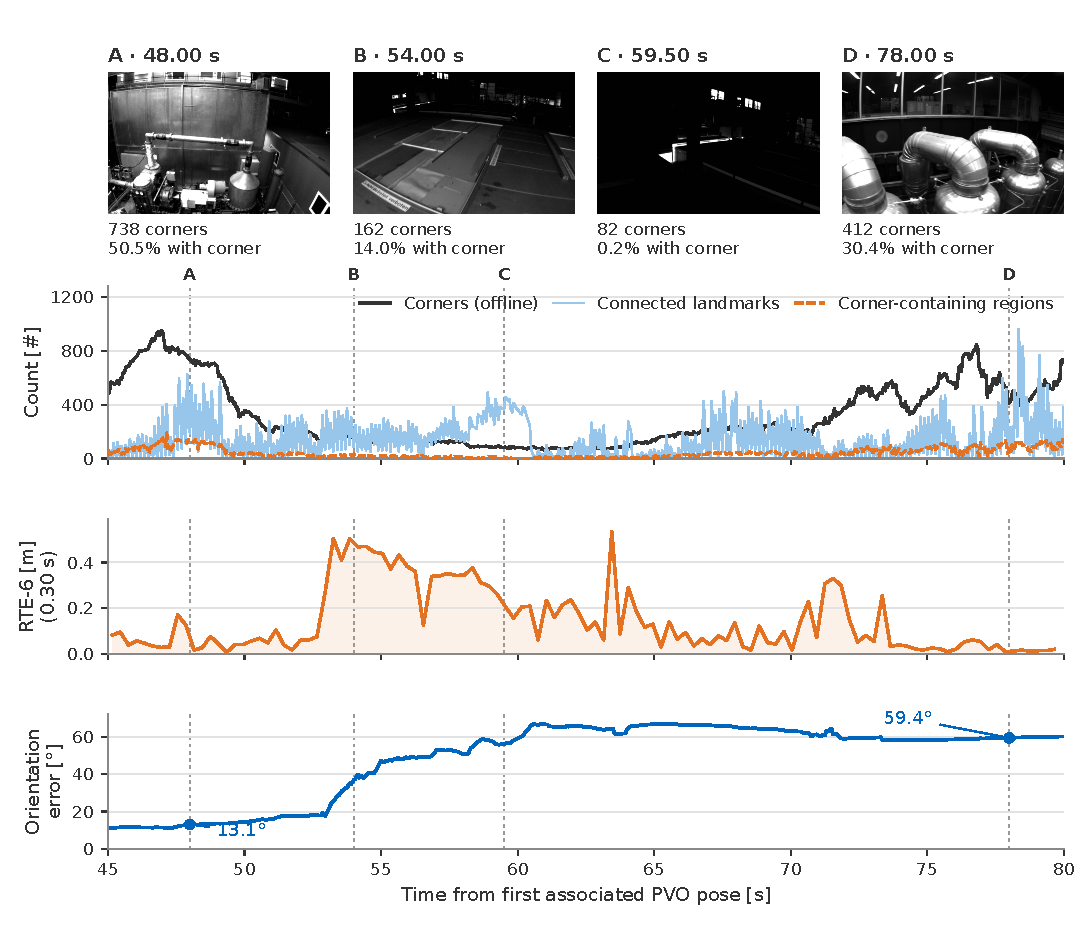
\includegraphics[width=\textwidth]{figures/evaluation/emh04-dark-scene-progression}
  \caption[Sustained drift on EMH04]{EMH04 before, during, and after sustained drift. Raw anchor-camera
  images are shown only for diagnosis. The synchronized traces distinguish
  changing image structure, local translation error, and persistent orientation
  error. Corner-containing regions are TEASER-stage MV destination blocks
  containing at least one offline Shi-Tomasi corner; the percentages divide
  their count by all logged TEASER-stage regions in each sampled frame.
  Connected IDs instead count observations linked to existing backend landmarks.
  Orientation error is aligned at the first pose, not over the full trajectory.}
  \label{fig:failure-emh04}
\end{figure}

The images and support measurements are consistent with less informative
codec predictions over broad surfaces and dark regions. The connection to
block-matching ambiguity follows the error-surface argument in
\autoref{eq:mv-error-hessian}~\cite{zhang2010subpixel,shi1994good}.
However, the recorded counts do not measure disparity accuracy or the spatial
rank of the retained point set. They cannot distinguish incorrect stereo
depth, temporal displacement bias, and unfavorable point geometry as the main
source of this episode. The fact that the paired absolute-residual run also
degrades in this interval provides an additional limit on its interpretation.

\subsection{A Brief Loss of Connections During Rapid Motion}

EMH03 contains a shorter event in which a six-frame interval reaches
\SI{0.4423}{\metre} RTE-6. It has an average of only 12.6 current IDs connected
to existing landmarks. A separate rapid-motion interval in the same sequence
has slightly greater translation and angular speed, yet its RTE-6 is only
\SI{0.0265}{\metre}. That interval retains 186.4 connected IDs on average.
The two image intervals contain similar numbers of detected corners, 656 and
670 per frame, respectively.

\begin{figure}[p]
  \centering
  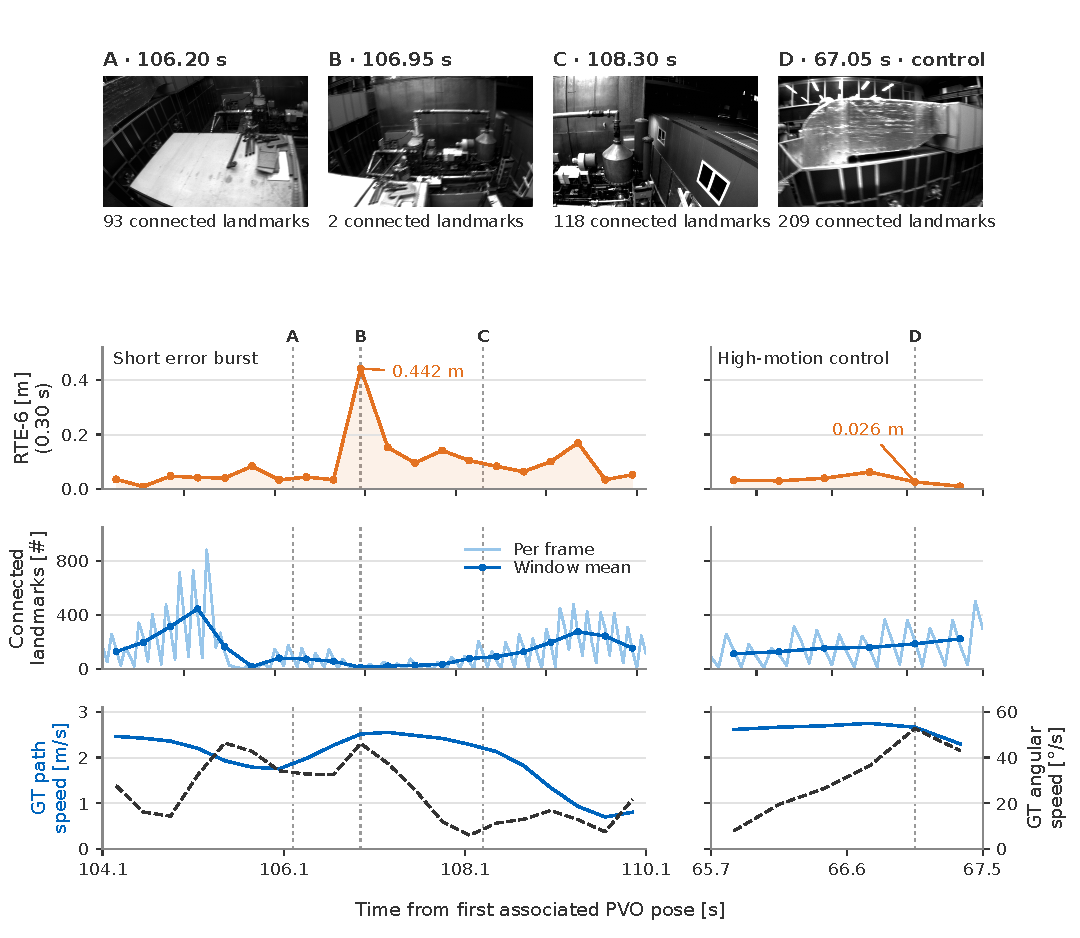
\includegraphics[width=\textwidth]{figures/evaluation/emh03-short-burst-and-motion-control}
  \caption[EMH03 error burst and rapid-motion comparison]{A short EMH03 error burst and a rapid-motion comparison interval.
  Connected IDs are current observations linked to existing backend landmarks.
  Similar image corner counts do not imply similar surviving temporal support;
  the faster comparison interval retains substantially more connections.}
  \label{fig:failure-emh03}
\end{figure}

This comparison separates the availability of visible structure from its
conversion into persistent observations. The failed interval is not simply
the faster or less corner-rich of the two. Its small connected set coincides
with a large local error, although the archived counters do not identify which
individual candidate losses produced that set. The absolute-residual run has
almost the same error in the burst, \SI{0.4397}{\metre}, which again indicates
that replacing rigid flow alone does not remove the event.

\subsection{Missing Temporal Observations, a Pose Jump, and a Stall}

EV103 illustrates a discontinuity rather than gradual drift. The view
approaches a bright window beside a broad dark partition. Visible corners and
emitted track IDs decrease. Inspection of the encoded streams also identifies
an I-frame in each direction at the endpoints of one temporal transition,
leaving no ordinary temporal MVs for that connection. Three frames later,
the estimated pose jumps by \SI{37.716}{\metre} and rotates by
\SI{174.42}{\degree} in one frame. Ground truth changes by only
\SI{0.050}{\metre} and \SI{0.77}{\degree}. At the jump, only two current IDs
are connected to existing landmarks; the optimizer records eight iterations,
six of them rejected.

\begin{figure}[p]
  \centering
  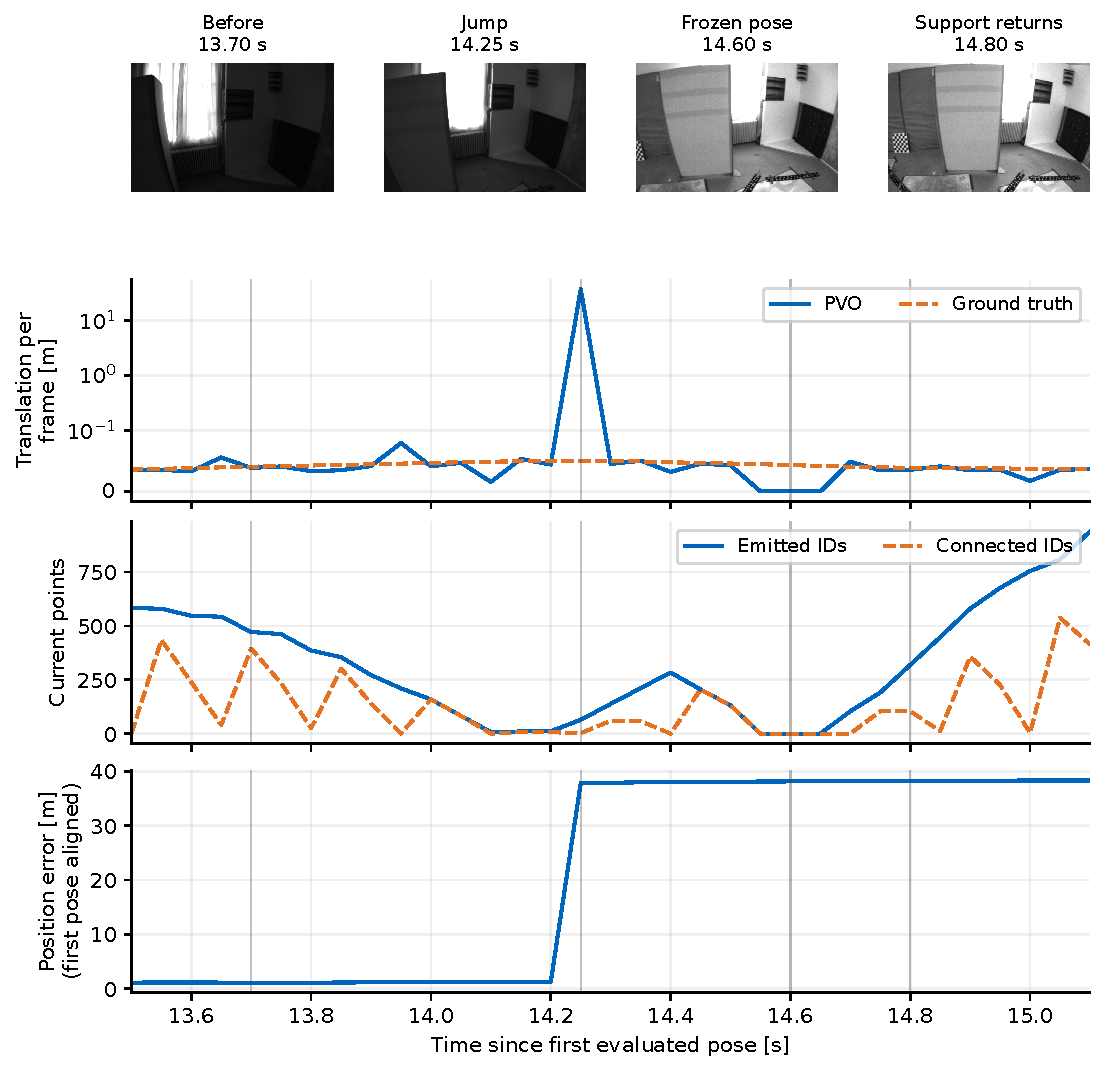
\includegraphics[width=\textwidth]{figures/evaluation/failure-ev103-jump}
  \caption[Catastrophic pose update on EV103]{EV103 around a catastrophic pose update. Per-frame translation uses
  a symmetric logarithmic axis so that ordinary motion, the large jump, and
  zero-motion outputs remain visible. The lower panels show the temporary loss
  of frontend support and the persistent position error after support returns.
  The sampled images are offline diagnostics.}
  \label{fig:failure-ev103}
\end{figure}

A subsequent transition again lacks temporal MVs in both directions. The
frontend then emits zero points for three consecutive frames and the pose
remains exactly unchanged, although ground truth moves approximately
\SI{0.04}{\metre} per frame. Image corners have already returned to at least
350 per frame. Raw MV candidates return after the missing transition, but no
candidate survives the logged stage requiring filtering and valid stereo at
both endpoints for the next two frames. These records locate the loss within
the processing chain; they do not isolate the median filter from stereo lookup
as its cause. Connections subsequently return, while the accumulated position
error remains approximately \SI{38}{\metre}.

The I-frames explain the observed absence of temporal vectors at particular
transitions, not the complete sequence of errors. The catastrophic update
itself occurs on a P-frame, and the shortage of usable observations extends
beyond the I-frame. The containing six-frame window contributes 98.6\% of
the full sequence's sum of squared six-frame translation errors. Its RTE-6 is
\SI{37.8510}{\metre}, compared with \SI{0.4066}{\metre} in the paired
absolute-residual run. This episode exposes a strong difference in how the
backends respond to the available observations; it does not show that every
large PVO error has the same origin.

\subsection{Low-Motion Errors and a Textured Counterexample}

EV202 contains consecutive estimated translations of \SI{1.117}{\metre} and
\SI{0.895}{\metre} while ground truth moves only \SI{0.013}{\metre} in each
frame. The images change little and show fabric-covered blocks, a plain wall,
and a small cart. Only three and two IDs, respectively, connect to existing
landmarks. At the first jump, 2919 raw MV regions and 541 stereo-valid temporal
candidates are still available, but only 25 reciprocal candidates and four
candidates passing the fitted rigid-model gate remain. This is another case
in which many initial observations do not translate into substantial temporal
support.

A later EV202 event provides a counterexample to using image corner count as a
sufficient indicator. A close, textured fabric surface dominates the view and
1640 corners are detected, yet the estimated translation is
\SI{0.752}{\metre} against a ground-truth step of \SI{0.015}{\metre}. Only six
IDs connect to existing landmarks. Conversely, a separate six-frame interval
with an average of 7.4 connected IDs has RTE-6 of only \SI{0.0376}{\metre}.
Neither high corner count nor low connection count alone determines the
outcome. Supplementary images and per-frame values are given in
\autoref{appendix:failure-episode-details}.

\subsection{What the Paired Residual Comparison Establishes}

\autoref{tab:episode-residual-comparison} compares identical timestamp
intervals from PVO, its absolute-residual ablation, and the frozen VOCA
OF-first reference. The two PVO runs share encoded inputs and frontend settings,
including the robust association procedure. EMH03's brief burst and EMH04's sustained error
remain under absolute reprojection. EV103's catastrophic amplification is much
smaller with absolute reprojection, as is EV202's textured-view error.
However, the EV202 jump at \SI{38.30}{\second} becomes larger. The observation
model thus changes the response to particular
correspondence sets without providing a universal safeguard. The low OF-first
errors on the same intervals show that the camera sequences still contain
information from which the richer reference can recover motion.

\begin{table}[htbp]
  \centering
  \caption[Observation-model comparison over failure episodes]{RTE-6 in metres; lower is better. Entries report
  RMSE over the listed non-overlapping windows. Absolute changes PVO's
  observation model; OF-first is the frozen pixel-refined reference. The
  EV202 middle jump is at \SI{38.30}{\second}, distinct from the later
  textured-view event.}
  \label{tab:episode-residual-comparison}
  \begin{tabular}{@{}lrrrr@{}}
\toprule
Episode & Windows & PVO [m] & Absolute [m] & OF-first [m] \\
\midrule
EMH03 burst & 1 & 0.4423 & 0.4397 & 0.0151 \\
EMH04 dark view & 26 & 0.3584 & 0.3719 & 0.0150 \\
EMH04 recovery & 23 & 0.0209 & 0.0270 & 0.0156 \\
EV103 jump & 1 & 37.8510 & 0.4066 & 0.0322 \\
EV202 early jumps & 1 & 1.3830 & 1.0851 & 0.0037 \\
EV202 middle jump & 1 & 1.1206 & 2.9941 & 0.0353 \\
EV202 textured view & 1 & 0.8402 & 0.2241 & 0.0019 \\
\bottomrule
\end{tabular}

\end{table}
